This section is separated to explain how clients can communicate 
with the services. 

Let's first take a look on an e-commerce platform design:

\begin{figure}[h]
\centering
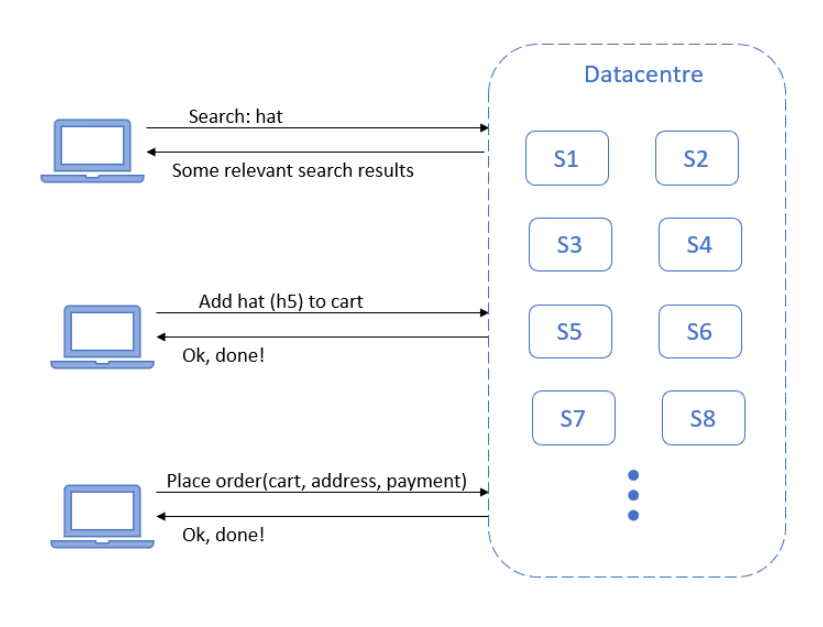
\includegraphics[width=0.8\linewidth]{figures/03_protocols_communication/e-commerce_platform.png}
\caption{e-commerce platform design}
\label{fig:ecommerce_platform_design}
\end{figure}



Say our user searches for a hat. Now the client will send a request 
to the server to search for hats and the server will respond with search 
results.

If a user wants to buy a hat, the client will send a request to the 
server to add the hat to the user's cart, and the server will respond 
with a confirmation.

If the user is happy with the items in their cart, on their action, 
the client will send the request to the server to place the order, 
and again, the server will respond with a confirmation.

In a real-world scenario, \hl{rather then talking about one specific server, 
the clients request will be send to a data center, where any server can 
pick the request}. However, irrespective of which server receives the request,
the response will be the same. Based on this flow, we can draw the following 
conclusions about this architecture:


\begin{itemize}
    \item It is client-driven. Only on the user's button click will 
    the client send the requests to the server, and the server will 
    only respond to these requests.
    \item It's a \textbf{request response model}. For every request the 
    server will respond with some information or simple confirmation. 
    \item There are occasional requests from clients, only one request 
    every few seconds based on the user's actions i.e from the client-side
    it is a \hl{low throughput system}. 
    \item It is a \hl{stateless} system, i.e irrespective to which server is 
    responding the answer will be always the same. 
\end{itemize}


\subsection{HTTP}
These requirements make this a perfect use case for HTTP(s) protocol. 
Although these days, most architectures on HTTP have moved to HTTPS, 
which is a more secure version of HTTP as it prevents man-in-the-middle
 attacks.

Now, when we are using HTTP, REST is usually the best API standard to 
follow as it is very widely used and very user friendly.

Let us look at an example for a REST request and response:

\begin{lstlisting}
    Request:
    Method: GET
    URL: https://www.twitter.com/user/{id}
    
    Response:
    Status: 200 OK
    Headers: <...>
    Body: {
        "userId": 1,
        "Email": "someone@example.com"
    }
\end{lstlisting}

The client makes a request to twitter.com over HTTPS to get 
information about a user with an id. In response, the server
sends a success status code along with the user's user id and email. 
As you can see, REST API standard is pretty much self-documenting,
which adds to its user friendliness.

Now let us look at an example of a chat application.

\begin{figure}[h]
\centering
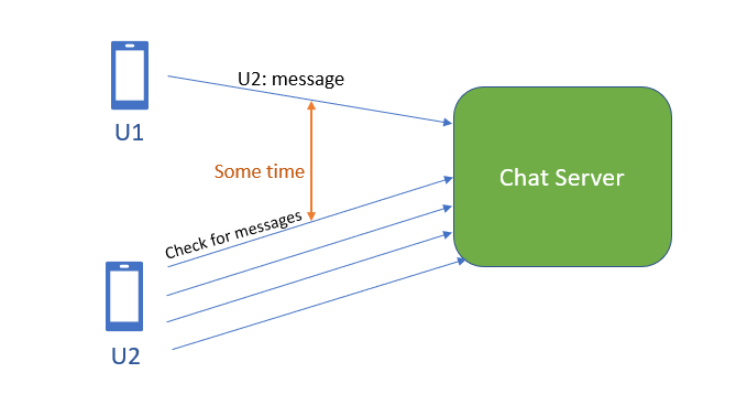
\includegraphics[width=0.8\linewidth]{figures/03_protocols_communication/chat_app.png}
\caption{Chat app}
\label{fig:chat_app}
\end{figure}

We know that the \hl{HTTP request is a client-driven protocol}, so the server
cannot intiate any contact with the client. It can only respond to the client upon
receiving a request. So when \texttt{U1} sends a message to \texttt{U2} via chat
server, \texttt{U2} doesn't receive the message until it asks the server to share 
any pending messages. \hl{This leads to a delay when receiving message}. \textit{It 
also makes the notification service impossible.}

A naive solution would be \texttt{U2} sending repeated requests to the server 
in the hope of receiving a message. But this consume too much resources and \hl{puts
a huge load on the chat server as it will receive a huge number of requests from all of 
its clients!}

Another solution woudl \texttt{polling}. The server could wait a few minutes before
responding to \texttt{U2}, thus increasing the chance of a message being received before
responding. But it's also not a very good solution. 

The best approach would be if the server could send a notification to the user every 
time there is a message. For this, we use a protocol called WebSocket.

\subsubsection{WebSocket}

A WebSocket connection \hl{is a persistent connection}. It is also a 
\hl{bidirectional protocol}, where communication can be initiated by 
the client or the server as long as there is an open connection. 
\hl{It is optimized for high-frequency communication}.

Let's look at how our chat application would work in the case of WebSocket protocol.

\begin{figure}[h]
\centering
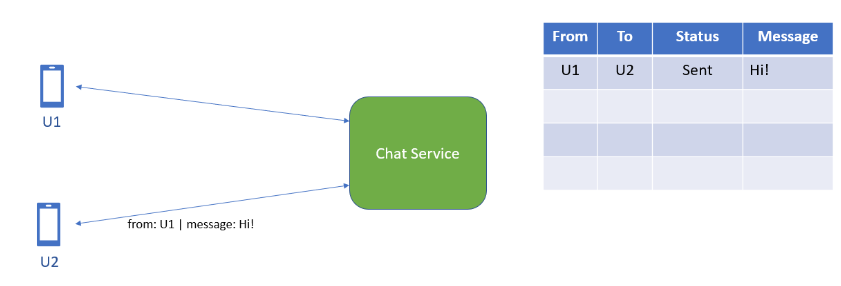
\includegraphics[width=0.8\linewidth]{figures/03_protocols_communication/websocket_protocol.png}
\caption{Chat app with websocket}
\label{fig:websocket_chat}
\end{figure}

First, \texttt{U1} and \texttt{U2} will establish HTTP connections with the chat server, 
which are then upgraded to a WebSocket connection. 
When \texttt{U1} sends a message for \texttt{U2} via the chat server, 
it will store the message along with its status, \texttt{RECEIVED}, let's say.

The chat server, if it has an open connection with \texttt{U2}, will 
then send the message to \texttt{U2} and update the status to \texttt{SENT}. 
If \texttt{U2} was not online and there was no open connection between 
\texttt{U2} and the server, the messages will be saved until \texttt{U2} 
comes online and requests the server to send all pending messages. 
The server will send all messages with the status \texttt{RECEIVED} and 
update the status to \texttt{SENT}.


As you can see, with this approach we have:

\begin{itemize}
    \item Reduced the latency, since the server can simply send the messages over an open connection
    \item Saved on CPU and bandwidth, as the client doesn't need to unnecessarily send requests 
    to the server and the server is not under unnecessary load.
    \item Provided better user experience. 
\end{itemize}

Even with the benefits, there is a high cost to using WebSockets; that is the cost of maintaining a 
persistent connection with millions of users.   

\subsubsection{Conclusion}
So how do we decide whether to use HTTP or WebSocket? Do we always go for 
Websocket then? Well, not really, as \hl{WebSocket is much more expensive than 
HTTP}. We can safely say, if the communication between client and 
server is at a lower throughput on the client-side, HTTP is the 
way to go. If the communication is always client-driven, WebSocket 
is not needed. Also, if you are on a tight budget, HTTP may be the 
better choice.

On the other hand, if the communication from the client is at a 
higher throughput, WebSocket may be a better option. If the 
communication can be driven by both client and server, WebSocket 
is the way to go. Although here comes the tradeoff between cost and
 performance. We must decide if the optimization is really worth the 
 huge cost of maintaining persistent connections with so many users.

 

